\documentclass{beamer}
\usepackage[T1]{fontenc}
\usepackage[utf8]{inputenc}
\usepackage{lmodern}
\usepackage[brazil]{babel}
\usepackage[labelformat=empty]{caption}
\usepackage{graphicx}
\usetheme{Luebeck}
\title[Padrão Model-View-Controller]{Padrão Model-View-Controller}
\author{Ana Luísa Losnak \and Luiz Armesto \and  Renan Fichberg}
\date{Novembro 4, 2014}
\institute{Instituto de Matemática e Estatística da Universidade de São Paulo (IME-USP)}

\expandafter\def\expandafter\insertshorttitle\expandafter{%
  \insertshorttitle\hfill%
    \insertframenumber\,/\,\inserttotalframenumber}

\begin{document}

\begin{frame}
\titlepage
\end{frame}

\begin{frame}
\frametitle{Introdução}
\begin{itemize}
	\item O que é um padrão?
	\item O padrão MVC
	\item Alguns \textit{frameworks} que usam MVC ou derivados
	\item Alguns padrões similares ao MVC
\end{itemize}
\end{frame}

%TODO: o que é um padrão (não há necessidade de dar exemplos. O tema por si só já é um exemplo)
\begin{frame}
\frametitle{O que é um padrão?}
	Em Engenharia de Software, um padrão de \textit{design} é uma solução geral que pode ser reutilizada para resolver um problema recorrente de um contexto específico de Design de Software
\end{frame}

\begin{frame}
\frametitle{O que é um padrão?}
\framesubtitle{Padrão de arquitetura}
  \begin{itemize}
  \item {Não é específico de uma arquitetura}
  \item {Solução geral que envolve a estrutura dos elementos de uma arquitetura de software}
  \end{itemize}
\end{frame}


%TODO: O padrão MVC
\begin{frame}
\frametitle{O padrão MVC}
\begin{itemize}
	\item Breve histórico
	\item Estrutura
	\item A tríade: os três componentes do MVC
	\item Padrões associados
	\item Por que usar?
\end{itemize}
\end{frame}

\begin{frame}
\frametitle{O padrão MVC}
% Essa explicação é boa para o MVC Model2. No MVC clássico o controller não serve de cola, ele serve para controlar o input.
	`An easy way to understand MVC: the model is the data, the view is the window on the screen, and the controller is the glue between the two.' \\
	\hfill \textit{- Connelly Barnes.}
\end{frame}


\begin{frame}
\frametitle{O padrão MVC}
\framesubtitle{Breve histórico}
\begin{itemize}
\item {Criado pelo cientista da computação norueguês Trygve Reenskaug}
\item {Originalmente para o \textit{framework} Smalltalk-80}
\item {Lançamento do \textit{paper} \textit{`A Cookbook for Using the Model-View-Controller User Interface Paradigm in Smalltalk -80'}, de Glenn Krasner e Stephen Pope, em Agosto/Setembro de 1988, no \textit{`Journal Of Object Oriented Programming'}}
\end{itemize}
\end{frame}

\begin{frame}
\frametitle{O padrão MVC}
\framesubtitle{Estrutura}
	O padrão divide uma aplicação em três componentes: o \textit{model}, as \textit{views} e os \textit{controllers}.

\begin{itemize}
	\item \textit{Model}: encapsula os dados e a funcionalidade
	\item \textit{View}: apresenta as informações para o usuário
  \item \textit{Controller}: trata a interação do usuário com o sistema
\end{itemize}

  As \textit{views} e os \emph{controllers} compreendem a interface de usuário.
\end{frame}

\begin{frame}
\frametitle{O padrão MVC}
\framesubtitle{A tríade - o Model}
\begin{center}
	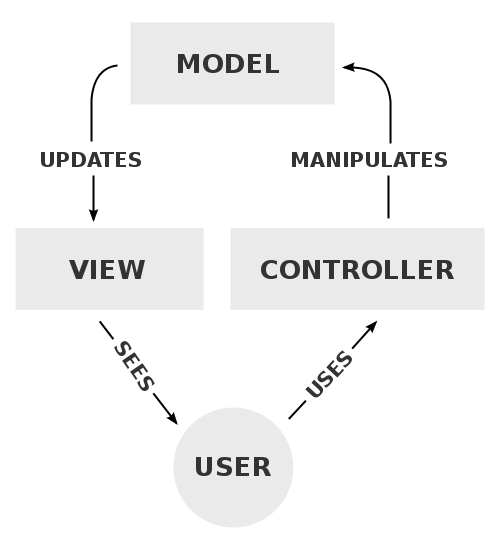
\includegraphics[scale=0.4]{MVC.jpg}
\end{center}
O \textit{Model}:
  \begin{itemize}
    \item {É responsável pela lógica da aplicação}
    \item {Independe da interface de usuário}
    \item {Apenas notifica as \textit{views} e os \textit{controllers} de alterações nos dados}
  \end{itemize}
\end{frame}

\begin{frame}
\frametitle{O padrão MVC}
\framesubtitle{A tríade - a View}
\begin{center}
	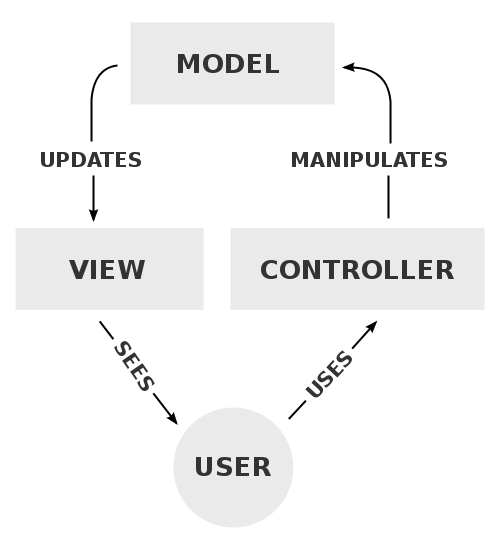
\includegraphics[scale=0.4]{MVC.jpg}
\end{center}
A \textit{View}:
\begin{itemize}
  \item {É responsável por qualquer saída de dados ao usuário}
  \item {Cria seu respectivo \textit{controller}}
  \item {Recebe dados do \textit{model}}
  \item {Podem existir várias \textit{views} para um mesmo \textit{model}}
\end{itemize}
\end{frame}

\begin{frame} [shrink=10]
\frametitle{O padrão MVC}
\framesubtitle{A tríade - o Controller}
\begin{center}
	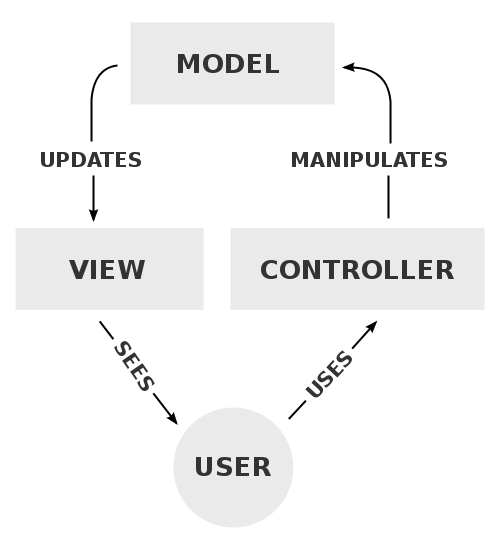
\includegraphics[scale=0.4]{MVC.jpg}
\end{center}
O \textit{Controller}:
\begin{itemize}
  \item {É responsável por qualquer entrada de dados na aplicação, como um \textit{click} do \textit{mouse} ou uso de teclas do teclado}
  \item {Trata as entradas de dados como eventos e os transforma em serviços}
  \item {Pode atualizar o estado do \textit{model} ou da \textit{view}}
\end{itemize}
\end{frame}

\begin{frame}
\frametitle{O padrão MVC}
\begin{center}
	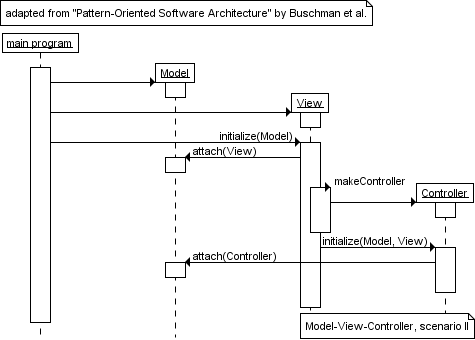
\includegraphics[scale=0.6]{MVCScenario.png}
\end{center}
\end{frame}

\begin{frame}
\frametitle{O padrão MVC}
\begin{center}
	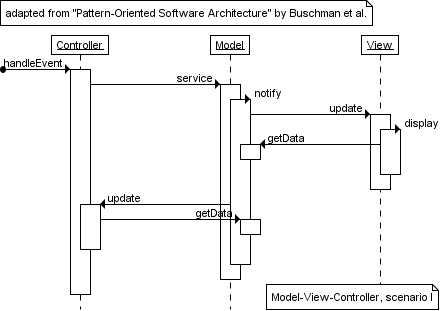
\includegraphics[scale=0.6]{MVCHandleEvent.png}
\end{center}
\end{frame}

\begin{frame}
\frametitle{O padrão MVC}
\framesubtitle{Padrões associados}
\begin{itemize}
	\item Observer: mantém as \textit{views} e os \textit{controllers} sincronizados com o \textit{model}
	\item Composite: permite a criação de \textit{views} compostas, contendo outras \textit{views}
	\item Strategy: permite a utilização de diferentes \textit{controllers} para uma mesma \textit{view}
\end{itemize}
\end{frame}

\begin{frame}
\frametitle{O padrão MVC}
\framesubtitle{Padrões associados - Observer}
\begin{itemize}
  \item {Peça-chave na implementação original do MVC}
  \item {\textit{Views} e \textit{controllers} sincronizados com \textit{models}}
  \item {O \textit{model} independe das \textit{views} e dos \textit{controllers}, reduzindo o acoplamento}
\end{itemize}
\end{frame}

\begin{frame}
\frametitle{O padrão MVC}
\framesubtitle{Padrões associados - Observer}
	\begin{center}
		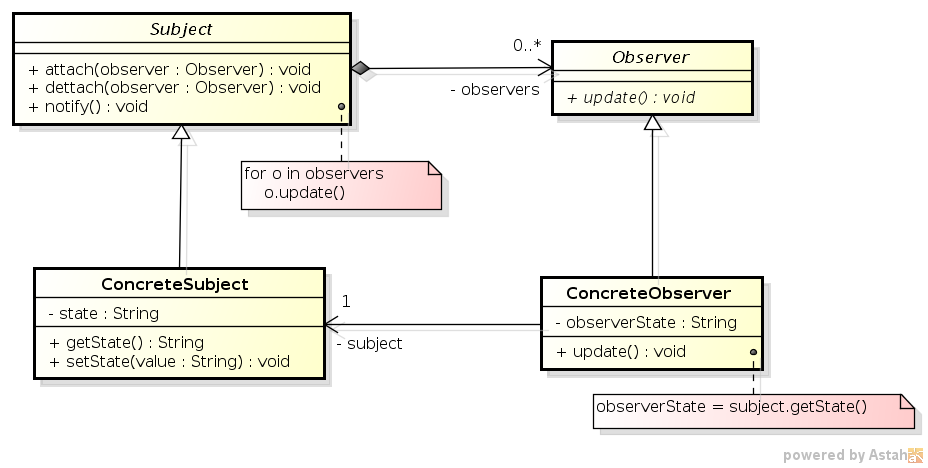
\includegraphics[scale=0.45]{Observer.png}
	\end{center}
\end{frame}

\begin{frame}
\frametitle{O padrão MVC}
\framesubtitle{Padrões associados - Observer}
\begin{center}
    \hspace{-1cm}
		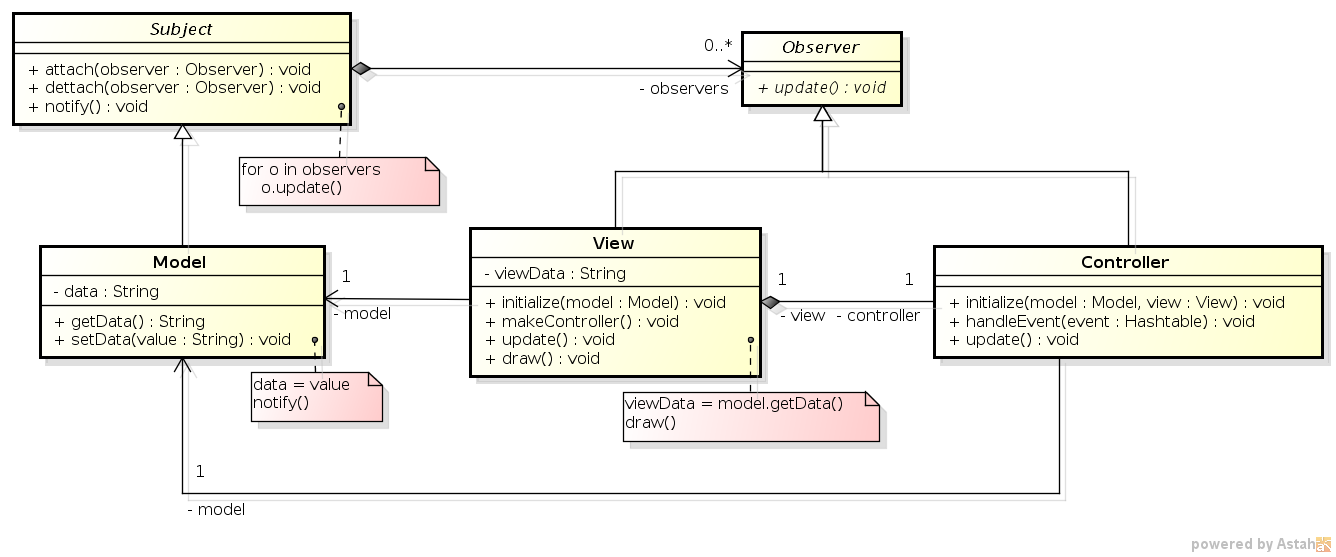
\includegraphics[scale=0.32]{ClassicMVC.png}
	\end{center}
\end{frame}

\begin{frame}
\frametitle{O padrão MVC}
\framesubtitle{Padrões associados - Composite}
  Permite a criação de \textit{CompositeViews}, tendo várias \textit{views} filhas responsáveis por cada elemento da interface de usuário.

  Exemplo: implementação de uma tela como uma \textit{CompositeView}, que possui uma \textit{view} para um campo texto, outra para um botão, outra para uma caixa de seleção, etc
\end{frame}

\begin{frame}
\frametitle{O padrão MVC}
\framesubtitle{Padrões associados - Strategy}
	Permite a utilização de diferentes modos de entrada e interação do usuário através da escolha de diferentes \textit{controllers} para uma mesma \textit{view}, bastando inicializar um ou outro \textit{controller} para comportamentos diferentes.

  Exemplo: um controller mais focado na interação utilizando o \textit{mouse} e outro focado na utilização de atalhos do teclado
\end{frame}

\begin{frame}
\frametitle{O padrão MVC}
\framesubtitle{Por que usar?}
\begin{itemize}
	\item Redução do entrelaçamento da interface de usuário com o núcleo funcional aumenta a flexibilidade
\begin{itemize}
  \item diversas interfaces para o mesmo comportamento da aplicação
  \item mudanças em uma interface não influenciam o comportamento da aplicação
\end{itemize}
	\item Diminue custos e propensão a erros na construção do sistema
	\item A separação de responsabilidades facilita a utilização de testes automatizados
\end{itemize}
\end{frame}


\begin{frame}
\frametitle{Alguns frameworks que usam MVC ou derivados}
\framesubtitle{}
	\textbf{ActionScript 3} - Cairngorm, PureMVC\\
	\textbf{ASP} - ASP Xtreme Evolution, Toika, AJAXED\\
	\textbf{Java} - Apache Struts, Tapestry, VRaptor, Spring MVC, JSF\\
	\textbf{Perl} - Catalyst\\
	\textbf{PHP} - CakePHP, CodeIgniter, LightVC, Symfony\\
	\textbf{Python} - Django\\
	\textbf{Ruby} - Rails\\
	\textbf{Smalltalk} - Smalltalk-80\\
	\textbf{Javascript} (server side) - Sails.js\\
	\textbf{Javascript} (client side) - AngularJs, Backbone.js, Ember.js\\
\end{frame}

\begin{frame}
\frametitle{Alguns frameworks que usam MVC ou derivados}
\framesubtitle{Rails}
\begin{itemize}
  \item {Rails não é MVC puro!}
  \item {Segue um modelo derivado, o \textbf{Model 2}}
\end{itemize}
\end{frame}

\begin{frame}
\frametitle{Alguns frameworks que usam MVC ou derivados}
\framesubtitle{Rails}
\begin{itemize}
  \item {MVC clássico: um \textit{model} pode notificar as \textit{views} sobre mudanças que aconteceram (a partir do padrão \textit{Observer})}
  \item {Estrutura no Rails: as \textit{views} não são notificadas pelo \textit{model}, mas recebem os dados do \textit{model} pelo \textit{controller}, como exibido no esquema abaixo:}
\end{itemize}
	\begin{center}
		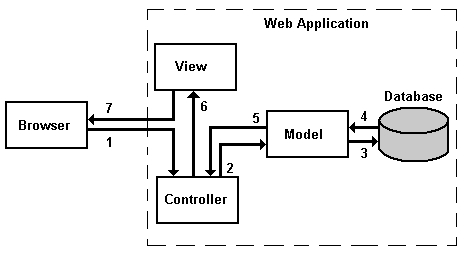
\includegraphics[scale=0.35]{RailsMVC.jpg}
	\end{center}
\end{frame}

\begin{frame}[shrink=5]
\frametitle{Alguns padrões similares ao MVC}
\framesubtitle{O Model 2}
	\begin{center}
		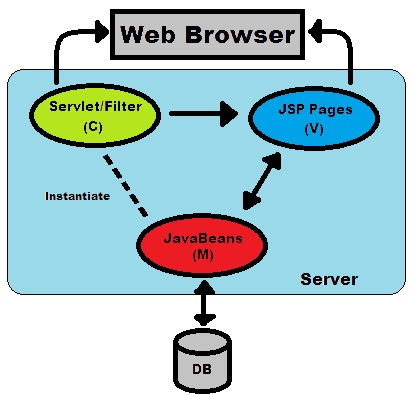
\includegraphics[scale=0.35]{Model2.jpg}
	\end{center}
  \begin{itemize}
  \item {As requisições do navegador do cliente são passadas para o \textit{controller}}
  \item {O \textit{controller} faz o que precisa para obter o conteúdo que deve ser exibido}
  \item {O conteúdo é colocado na requisição, freqüentemente como um JavaBean, e é repassado para uma \textit{view}, que o renderiza}
\end{itemize}
\end{frame}

\begin{frame}
\frametitle{Alguns padrões similares ao MVC}
\framesubtitle{O Hierarchical Model–View–Controller (HMVC)}
  Similar ao padrão \textit{Presentation–Abstraction–Control (PAC)}, o HMVC surgiu como uma tentativa de resposta aos problemas de escalabilidade.
	\begin{center}
		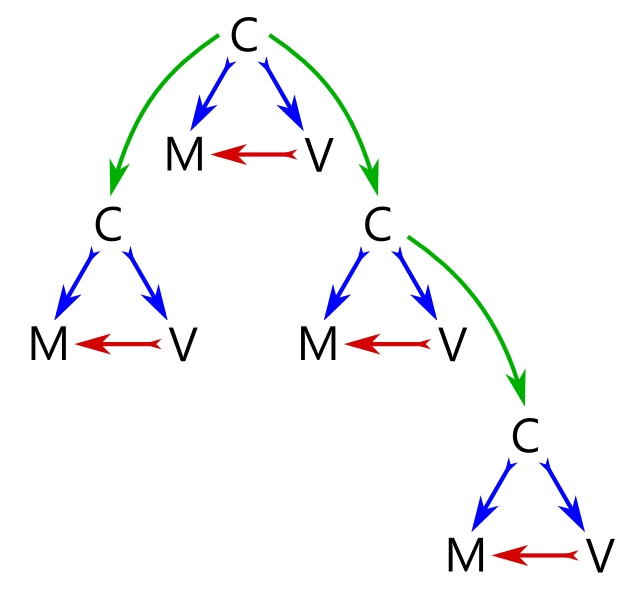
\includegraphics[scale=0.175]{HMVC.jpg}
	\end{center}
	Cada tríade funciona independentemente e uma tríade pode fazer requisição de acesso a outra a partir dos seus \textit{controllers}.
\end{frame}

\begin{frame}
\frametitle{Alguns padrões similares ao MVC}
\framesubtitle{MVC versus HMVC: algumas diferenças}
	\begin{itemize}
	\item MVC é mais simples.
	\item HMVC é mais escalável.
\end{itemize}
\end{frame}

\begin{frame}
\frametitle{Alguns padrões similares ao MVC}
\framesubtitle{O Movel-View-Adapter (MVA)}
	\begin{center}
		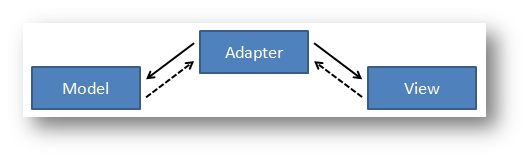
\includegraphics[scale=0.4]{MVA.jpg}
	\end{center}
	Na imagem, as linhas tracejadas representam comunicação indireta, através do uso do padrão \textit{Observer}, enquanto as linhas contínuas são relações diretas.
\end{frame}

\begin{frame}
\frametitle{Alguns padrões similares ao MVC}
\framesubtitle{MVC versus MVA: algumas diferenças}
\begin{itemize}
	\item Desacoplamento total do \textit{model} e da \textit{view} no MVA
	\item Toda a dinâmica da aplicação é centralizada no \textit{adapter}
\end{itemize}
\end{frame}

\begin{frame}
\frametitle{Alguns padrões similares ao MVC}
\framesubtitle{O Movel-View-Presenter (MVP)}
	\begin{center}
		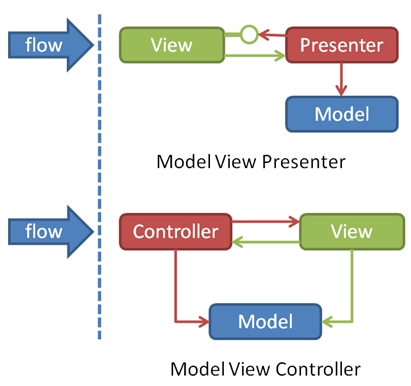
\includegraphics[scale=0.3]{MVP.jpg}
	\end{center}
	\begin{itemize}
    \item A \textit{view} é a responsável por manipular os eventos da interface de usuário, função do \textit{controller} no MVC tradicional
    \item O \textit{presenter} só interage com a \textit{view} por meio de uma interface, facilitando a realização de testes de unidade automatizados
    \item O \textit{presenter} age sobre o \textit{model} e a \textit{view}, atualizando e recuperando dados do \textit{model} e passando-os já preparados para a \textit{view}, que apenas deverá exibi-los da maneira esperada
\end{itemize}
\end{frame}

\begin{frame}
\frametitle{Alguns padrões similares ao MVC}
\framesubtitle{MVC versus MVP: algumas diferenças}
\begin{itemize}
	\item A \textit{view} está menos amarrada ao \textit{model} no MVP. Amarrá-los é tarefa do \textit{presenter}.\\
	\item Mais facilidade para realizar testes de unidade no MVP.\\
	\item \textit{Views} complexas podem ter múltiplos \textit{presenters}.
	\item No MVC, a parte lógica deve sempre ficar completamente isolada da \textit{view}.
	\item No MVC, o \textit{controller} é baseado em comportamentos e pode ser compartilhado através das \textit{views}.
\end{itemize}
\end{frame}

\begin{frame}
\frametitle{Referências}
\begin{itemize}
	\item GAMMA, Erich; HELM, Richard; JOHNSON, Ralph; VLISSIDES, John; \textit{Design Patterns: Elements of Reusable Object-Oriented Software}. 1st Edition. Addison-Wesley. 1995.
	\item SCHMIDT, Douglas C; STAL, Michael; ROHNERT, Hans; BUSCHMANN, Frank; \textit{Pattern-Oriented Software Architecture, Volume 2: Patterns for Concurrent and Networked Objects}. 2nd Edition. John Wiley and Sons. 2000.
	\item FOWLER, Martin; \textit{Patterns of Enterprise Application Architecture}. 1st Edition. Addison-Wesley. 2002.
	\item en.wikipedia.org/
\end{itemize}
\end{frame}

\end{document}
